\documentclass[12pt,a4paper]{article}
\usepackage[utf8]{inputenc}
\usepackage[T1]{fontenc}
\usepackage{amsmath}
\usepackage{amsfonts}
\usepackage{amssymb}
\usepackage{lipsum}
\usepackage{textcomp}

\usepackage{makecell} % linebreak dans une cellule
\usepackage{multicol} % twocols localement
\usepackage{vwcol} % idem mais avec largeur variable
\usepackage{color, colortbl} % colorer les tableaux
\usepackage{enumitem} % utiliser des lettres pour énumérer
\usepackage{wrapfig} % insérer des images dans dutexte
\usepackage{dashundergaps} % transformer du texte en ________
\usepackage{MnSymbol,wasysym} % smileys
\usepackage{ifthen}
\usepackage{soul} % teste barré \st

% --- geometry ---
\usepackage{geometry}
\geometry{legalpaper, margin=2cm}
% ---

% --- xcolor ---
\usepackage{xcolor}
\definecolor{lightgray}{gray}{0.9}
% ---

% --- tcolorboxes ---
\usepackage[most]{tcolorbox}
\newtcolorbox{definition}[2][]{%
  attach boxed title to top left
               = {yshift=-8pt},
  colback      = white,
  colframe     = gray,
  fonttitle    = \bfseries,
  colbacktitle = gray,
  title        = #2,#1,
  enhanced,
}
% ---


\renewcommand{\baselinestretch}{1.15} % augmenter l'interligne

\dashundergapssetup{
	teacher-gap-format=underline,
	gap-widen
}



\author{Paul Clavier}
\title{Chapitre 2 - Les nombres décimaux}

\begin{document}

% --- Section & subsection renum ---
\renewcommand\thesection{\Roman{section}}
\renewcommand\thesubsection{\arabic{subsection}}
% ---

% --- Selection manuelle de la version ---
%\TeacherModeOn
% ---

% --- Selection automatique de la version ---
\ifdefined\isprof
	\TeacherModeOn
\fi

% ---



\begin{center}
	\fbox{\parbox{\dimexpr\linewidth-2\fboxsep-2\fboxrule\relax}{\centering\huge Chapitre 3 - Premiers éléments de géométrie et grandeurs usuelles}}
\end{center}

\section{Vocabulaire de base}

\subsection{Le point}

\begin{definition}{Définition}
Le point, selon Euclide, est ce qui n'a aucune partie. On peut aussi dire plus simplement qu'un point ne désigne pas un objet mais un emplacement. Il n'a donc aucune dimension, longueur, largeur, épaisseur, volume ou aire. Sa seule caractéristique est sa position. On dit parfois qu'il est « infiniment petit ».
\end{definition}
Un point est noté comme il suit:\\
\begin{minipage}{0.2\textwidth}
\begin{center}
\includegraphics[scale=1]{img/point-A.png}
\end{center}
\end{minipage}
\begin{minipage}{0.8\textwidth}
Remarques:
\begin{itemize}
\item On le note souvent par une croix «+» qui représente l'intersection de deux droites imaginaires
\item On le nome d'une lettre majuscule
\end{itemize}
\end{minipage}

\subsection{Droite, demi-droite et segment}

\begin{tabular}{|c|c|c|}
\hline 
Notation & Signification & Figure \\ 
\hline 
\gap*{$[AB]$} & \thead{« Segment $[AB]$ »\\C'est le segment d'extrémités les points $A$ et $B$} & \thead{\gap*[b]{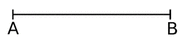
\includegraphics[scale=0.9]{img/segment-AB.png}}}  \\ 
\hline 
\gap*{$(AB)$} & \thead{« Droite $(AB)$ »\\C'est la droite qui passe par les points $A$ et $B$} & \thead{\gap*[b]{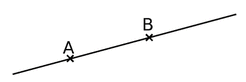
\includegraphics[scale=0.6]{img/droite-AB.png}}} \\ 
\hline 
\gap*{$[AB)$} & \thead{« Demi-droite $[AB)$ »\\ C’est la demi-droite d’origine $A$ passant par le point $B$.} & \thead{\gap*[b]{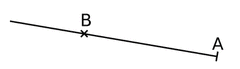
\includegraphics[scale=0.6]{img/demidroite-AB.png}}} \\ 
\hline 
\thead{\gap*{$A\in (d)$}\\ \gap*{$B\nin (d)$}} & \thead{Le point $A$ appartient à la droite $(d)$.\\ Le point $B$ n’appartient pas à la droite $(d)$}. & \thead{\gap*[b]{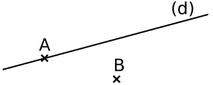
\includegraphics[scale=0.6]{img/point-appartenence.png}}} \\ 
\hline 
\end{tabular} 

\subsection{Points alignés}

\begin{minipage}{0.4\textwidth}
\begin{definition}{Définition}
Trois points sont \gap*{alignés} s'ils appartiennent à une même droite.
\end{definition}
\end{minipage}
\begin{minipage}{0.25\textwidth}
\textbf{Exemple}:
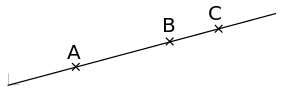
\includegraphics[scale=0.6]{img/alignement.png} 
\end{minipage}
\begin{minipage}{0.4\textwidth}
Les points $A$, $B$ et $C$ sont \gap*{alignés}.
\end{minipage}

\section{Droites sécantes}

\begin{definition}{Définition}
Deux \gap*{droites sécantes} sont deux droites qui se coupent en un point. Ce point est appelé \gap*{point d'intersection}.
\end{definition}

\textbf{Exemple}:\\
\begin{center}
\begin{minipage}{0.4\textwidth}
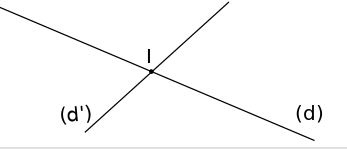
\includegraphics[scale=0.8]{img/secantes.png}
\end{minipage}
\begin{minipage}{0.4\textwidth}
Le point $I$ est le \gap*{point d'intersection} des droites $(d)$ et $(d')$.
\end{minipage}
\end{center}

\section{Longueur d'un segment}

\begin{tabular}{|c|c|c|}
\hline 
Notation & Signification & Figure \\ 
\hline 
\gap*{$AB$} & C'est la \gap*{longueur} du segment $[AB]$. & \thead{\gap*[b]{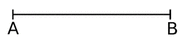
\includegraphics[scale=0.6]{img/segment-AB.png}}\\\gap*{$AB=3cm$}} \\ 
\hline 
\end{tabular}\\

\textbf{Remarque}: Une mesure de longueur a toujours une unité (m, cm, km, ...).

\section{Milieu d'un segment}
\begin{definition}{Définition}
Le \gap*{milieu} du segment $[AB]$ est le \gap*{point} du segment $[AB]$ qui est équidistant (à la même distance) des points $A$ et $B$.
\end{definition}

\textbf{Exemple}: Trace un segment $[RT]$ de longueur 6cm puis construis son milieu $A$.

\begin{tabular}{|c|c|c|}
\hline 
\thead{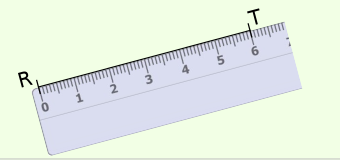
\includegraphics[scale=0.5]{img/milieu-1.png}} & \thead{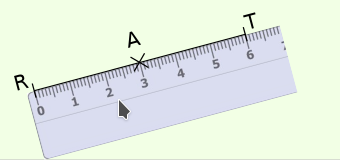
\includegraphics[scale=0.5]{img/milieu-2.png}} & \thead{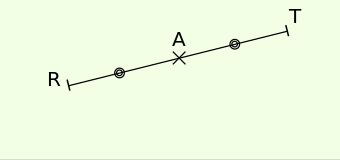
\includegraphics[scale=0.5]{img/milieu-3.png}} \\
\hline 
\thead{On trace le segment $[RT]$\\de longueur 6cm} & \thead{On place le point $A$ à 3cm du\\point $R$ sur le segment $[RT]$} & \thead{On code les segments $[RA]$ et $[AT]$\\qui sont de même longueur avec un\\même symbole.} \\ 
\hline 
\end{tabular} 


\end{document}